

\documentclass[12pt, a4paper]{article}


\usepackage{fancyhdr, enumerate}
\usepackage{amssymb}
\usepackage{geometry, amsmath, amsfonts, float, graphicx}
\usepackage{gensymb}
\usepackage{hyperref, listings}
\usepackage{matlab-prettifier}
\usepackage{caption}
\def\Z{\mathbb Z}
\geometry{
	top=0.9in,           
	inner=0.6in,
	outer=0.6in,
	bottom=2in,
	tmargin= 10ex,       
	headsep=0.6cm,          
}
\pagestyle{fancy}

\fancyhead{}
\fancyfoot{}

\fancyhead[L]{Bioen 316 AC \\Homework 6\\ May 31, 2019}
\fancyhead[R]{Skyler Hallinan\\ hallisky@uw.edu \\ 1732227}

\lstMakeShortInline[style=Matlab-editor]"
\begin{document}
\vspace*{-3mm}
\section*{Problem 1} 
Brain rhythms are commonly known by Greek letters, which appear here in order of
their frequency ranges: Delta (1 – 4 Hz), Theta (4 – 9 Hz), Alpha (8 – 12 Hz), Beta
(12 – 20 Hz), and Gamma ($>$30 Hz). These rhythms usually appear in the same
signal and must be extracted by filtering. Your goal is to create a discrete-time
(digital) finite impulse response band pass filter that will keep the beta waves and
attenuate the rest of the signal. \\ \\
``Creating an FIR filter'' means coming up with the sequence of coefficients that are
convolved with a discrete signal to filter that signal. Task 1 produces filter
coefficients $h(n\cdot t_s)$ on paper rather than using \textsc{Matlab}. It is probably easier to
work in continuous time and frequency until you have a complete filter function
h(t), and then substitute $t = n \cdot t_s$. You may write the answer to task 1 as the product
of three functions. In task 2 we will apply the filter to an EEG signal using \textsc{Matlab}.
\begin{enumerate}[(a)]
\item Determine the cutoff frequency of a low pass filter that will, after shifting in the
frequency domain, produce the proper bandwidth for the band pass filter. Use this
cutoff frequency and the Fourier transform pairs below to derive $h_{LPF}(t)$. \\ \\
\textbf{Answer: } \\
We first design the low-pass portion of our bandpass filter in the frequency domain. We want this low-pass filter to satisfy the appropriate width requirements of the desired bandpass filter (after shifting). To do this, we need a cutoff frequency $\omega_0$, from which we will create a rectangular pulse from $-\omega_0$ to $\omega_0$, with height 1. Since we are in the frequency domain, we are attenuating all frequencies outside this pulse, and retaining frequencies in the rectangular pulse. \\ \\
We want to keep the $\beta$ rhythms, which lie between 12-20 Hz. Using the conversion $\omega = 2 \pi f$, we see that the $\beta$ frequency range is between $24 \pi$ to $40 \pi \ \frac{rads}{sec}$. We see that the difference between these, the bandwidth, is $ 16 \pi \frac{rads}{sec}$. We want our low-pass filter to have the same bandwidth (but centered at 0), so we set the cutoff frequency $\omega_0$ to 8$\pi \ \frac{rads}{sec}$ so that the bandwidth, $2\omega_0$, is equal to $16\pi$, our desired bandwidth. \\ \\
Thus, our low pass filter is a rectangular pulse of height 1 over $ - \omega_0 < \omega < \omega_0$ which is equal to$ -8\pi < \omega < 8 \pi$. Then, we convert from frequency to time domain by using the relation between a rectangular pulse and the sinc function. In the time domain, this is written as $h_{LPF}(t) = \frac{\sin(8\pi t)}{\pi t}$. 
\item Multiply $h_{LPF}(t)$ by a function such that their product, $h_{BPF}(t)$, would perform band
pass filtering if convolved with a continuous signal. Describe how this multiplication
modifies the filter spectrum, i.e. how it changes the pass band(s). \\ \\
\textbf{Answer: } \\
In order to create a band-pass filter, we must shift the center of our low-pass filter from 0 $\frac{rads}{sec}$ to the middle of our desired frequency range. We can do this by multiplying our LPF by $\cos(x t)$, where $x$ is the desired center of the filter in $\frac{rads}{sec}$. Since our desired range is $12 -20$ Hz, which is $24\pi$ to $40 \pi \frac{rads}{sec}$, the center frequency is $32 \pi \frac{rads}{sec}$. \\ \\
Therefore, we multiply our previous low-pass filter by $\cos(32\pi t)$. This shifts the center of our LPF (which was previously centered at 0) to $32 \pi$, and retains the bandwidth of $16 \pi$. This therefore creates a BPF; our pass bands are now at width $16 \pi$ and centered at $32 \pi$, which was our goal in making our BPF. \\ \\
Our finally equation is $h_{BPF}(t) = \frac{\cos(32\pi t)\sin(8\pi t)}{\pi t}$
\item Set limits on the time span of $h_{BPF}(t)$ and describe how this truncation of $h_{BPF}(t)$
affects its magnitude spectrum. I recommend extending $h_{BPF}(t)$ out to the third or
fourth zero in $h_{LPF}(t)$, but Note 2 shows another option. The exact width is up to you. \\ \\
\textbf{Answer: } \\
We truncate our filter by finding the zeros of our LPF. We find the fourth zero in $h_{LPF}(t)$:
\begin{align*}
h_{LPF}(t) &= \frac{\sin(8\pi t)}{\pi t} = 0 \\
t_n &= \frac{n}{8}, \quad n \neq 0, \quad n \in \Z \\
t_4 &= \frac{4}{8} = \frac{1}{2} s
\end{align*}
Then we see that we can redefine our function as:
\begin{align*}
h_{BPF}(t) &= \frac{\cos(32\pi t)\sin(8\pi t)}{\pi t}, \quad \frac{1}{2} \leq t \leq \frac{1}{2}, \quad T = 1
\end{align*}
Truncation of our filter in the time domain is the same as convolution in the frequency domain. Therefore, by truncating our filter, we introduce pass-band ripples, which leads to inconsistent filtering. Instead of having smooth borders in our frequency domain to create the rectangular pulse between defined frequencies at constant height, the borders have ``ripples'', which are non-zero frequencies at the edges of the pulse, and slightly higher magnitudes of frequency at the edges of the rectangle; these ripples ``decay'' with distance away from the edge (their magnitude decreases). Therefore our magnitude spectrum is not a rectangle anymore; there has been noisy ripples introduced, which creates non-zero frequencies outside of our desired pass-band frequency rectangle in the form/shape of a ripple. Therefore, our filtering is not as accurate anymore.
\item Multiply the truncated $h_{BPF}(t)$ by an appropriate smoothing window to create
$h_{SMOOTH-BPF}(t)$. Describe how this multiplication improves the situation in the
frequency domain. \\ \\
\textbf{Answer: } \\
We choose our time domain to be from $-\frac{T}{2}$ to $\frac{T}{2}$. Therefore, our smoothing Hamming Window is $w(t) = 0.54 + 0.46\cos(\frac{2\pi t}{T})$
\begin{align*}
w(t) &= 0.54 + 0.46 \cos \left(\frac{2 \pi t}{T}\right), \quad -\frac{T}{2} \leq t \leq \frac{T}{2}, \quad T = 1s \\
h_{SMOOTH-BPF}(t) &= h_{BPF}(t)\cdot w(t)\\
h_{SMOOTH-BPF}(t) &= \frac{\cos(32\pi t)\sin(8\pi t)}{\pi t}\left[0.54 + 0.46 \cos \left(2\pi t\right)\right], \quad -\frac{1}{2} \leq t \leq \frac{1}{2}
\end{align*}
Multiplying by this smoothing Hamming Window removes discontinuities from our filter (in the time domain), and instead makes the endpoints line up smoothly, end to end (time domain). Depending on the accuracy and detail of the filter, this filter will remove most to all of the rippling effects in the frequency domain that were introduced by time-domain truncation step previously. Rather than having ripples near the edges of our rectangular pass band in the frequency domain, we will have a well-defined rectangle. This improves the accuracy of our filter in removing undesired frequencies, as we have a well-defined pass band rectangle.
\item
Read Task 2(a). Use the time values in the PhysioBank data to determine the EEG
sampling frequency. Use this sampling frequency to make the substitution $t = n\cdot t_S$. \\ \\
\textbf{Answer: } \\ From the imported data, we see that the sampling rate is $t_s = \frac{1}{160} \frac{secs}{sample}$, as we have 10 seconds represented by 1600 points ($\frac{10}{1600} \to \frac{1}{160}$). Thus, we make the substitution $t = n\cdot t_s = \frac{n}{160}$ for all $t$ in our BPF (including the limits), and simplify:
\begin{align*}
%w(n) &=  \frac{\cos(\frac{32 \pi}{160} n)\sin(\frac{8 \pi}{160} n)}{\pi t}\left[0.54 + 0.46 \cos \left(\frac{2\pi}{160} n)\right)\right], \quad -80\leq n \leq  80 \\
h(n) &=  \frac{\cos(32 \pi \cdot \frac{n}{160})\sin(8 \pi\cdot \frac{n}{160})}{\pi \cdot \frac{n}{160}}\left[0.54 + 0.46 \cos \left(2\pi \cdot \frac{n}{160})\right)\right], \quad -80\leq n \leq  80, \quad n \in \Z \\
 &=  160\frac{\cos(\frac{\pi}{5} n)\sin(\frac{\pi}{20} n)}{n\pi}\left[0.54 + 0.46 \cos \left(\frac{\pi}{80} n)\right)\right], \quad -80\leq n \leq  80, \quad n \in \Z
\end{align*}
We have successfully rewritten our smoothed BPF in terms of $n$ rather than $t$.
\end{enumerate}
\pagebreak
\section*{Problem 2}
Download one trace of 10-second data from the EEG Motor Movement/Imagery Datset (in PhysioBank ATM). Create the filter coefficients based on the solution generated in Problem 1, and apply it to this signal. Plot the time and frequency domain of the original and the filtered signal. \\ \\
\textbf{Answer: } \\ 
We downloaded the ``cz'' trace of sample 1 from the directory, created our filter in \textsc{Matlab}, and convolved our original signal with the filter to look only at $\beta$ Wave frequencies. See the annotated code for a more detailed annotation of the steps.
\begin{figure}[H]
\centering
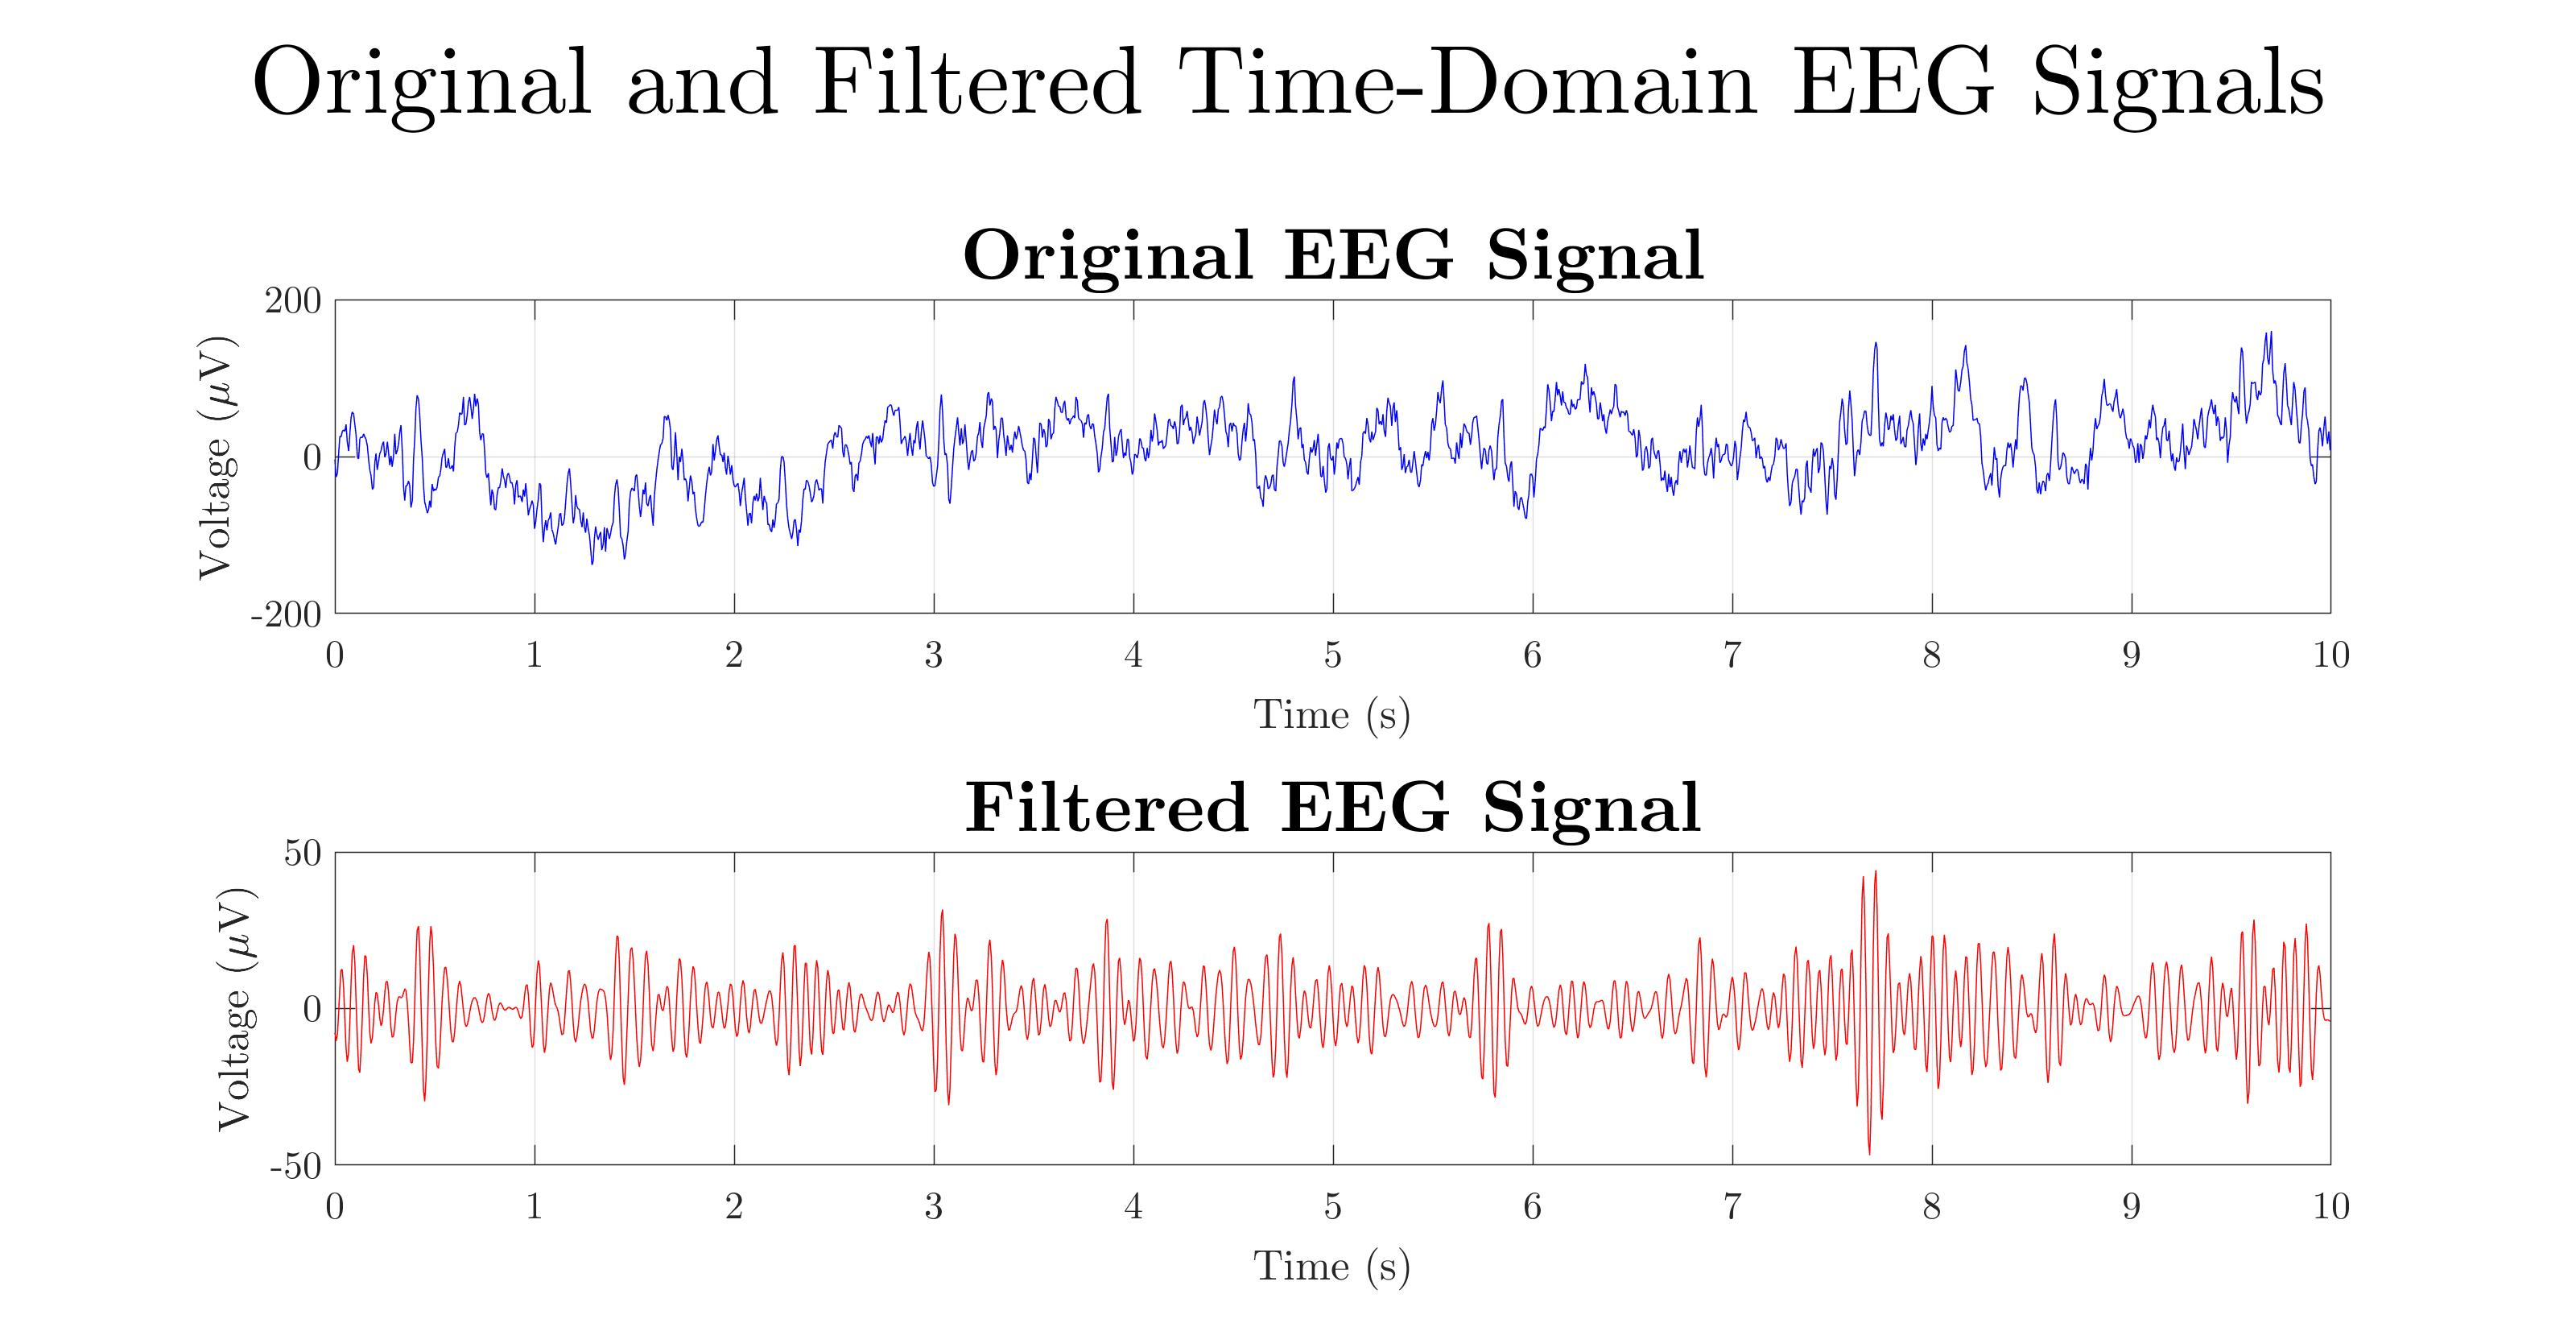
\includegraphics[width=\textwidth]{time}
\caption{Original vs Filtered EEG data}
\end{figure}
\noindent We see that our filtered signal has changed from our original signal.
\begin{figure}[H]
\centering
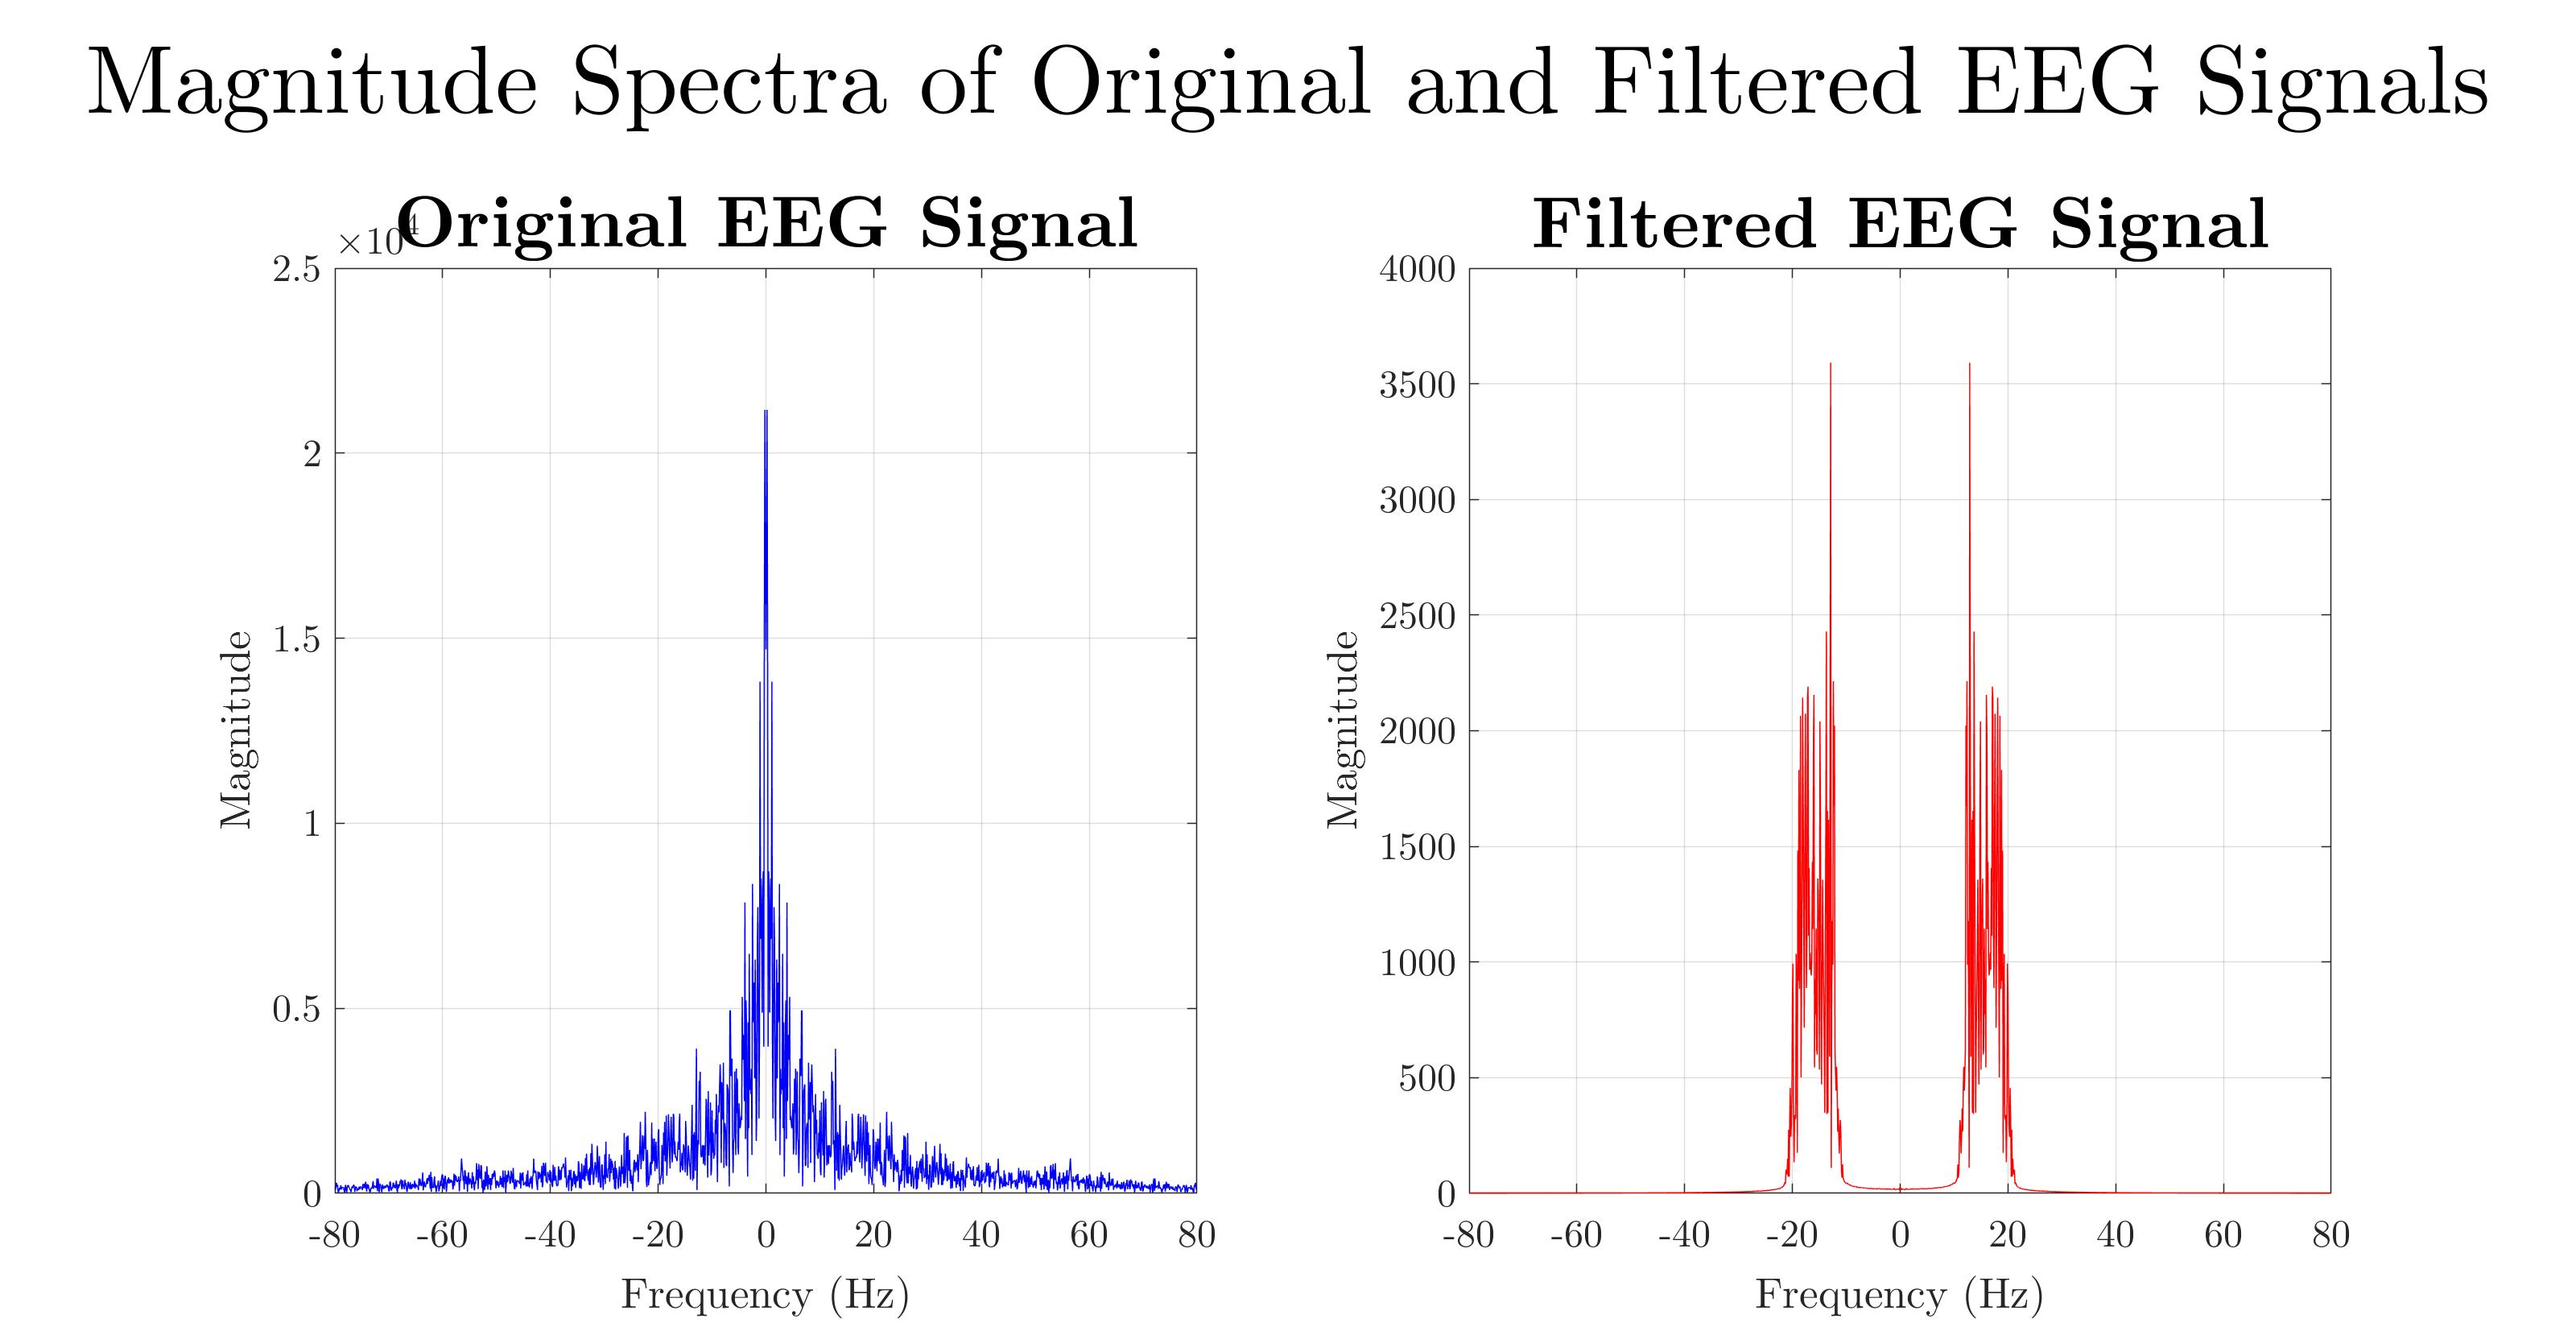
\includegraphics[width=\textwidth]{mag}
\caption{Original vs Filtered EEG Magnitude Spectra}
\end{figure}
\noindent We see that we have sucessfully captured frequencies in our desired range (12-20Hz), while attenuating the rest, from original to filtered signal.

\pagebreak
\section*{\fontsize{19}{15}\selectfont Appendix A}
\subsection*{MATLAB code}
\lstinputlisting[style=Matlab-editor]{hw6.m}
\end{document}